\chapter{Présentation des noeuds}\label{chapter:noeuds}

	\section{Le prélude}
        Le prélude permet d'afficher des paragraphes au début du livre, ajouter des items/skills à prendre/acheter, ainsi que de créer son personnage. Pour accèder au prélude, l'utilisateur doit d'abord selectionner le mode 
\includegraphics[height=10pt]{img/modeSelected.png}, puis double cliquer sur le prélude, situer dans la fenêtre d'édition, défini par un carré rose fushia.
		Trois onglet sont alors afficher. Le premier permet de définir le texte à afficher au tout début. Le deuxième permet de définir les items à prendre et/ou à acheter ainsi que les compétences disponibles au debut du livre. Et enfin, le dernier onglet concernet la création du personnage.

		\subsection{Création du personnage}
			Cette onglet à un bouton 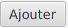
\includegraphics[height=10pt]{img/ajouterBouton.png}, permettant ainsi d'éditer d'autre paragraphes à afficher, avant le commencement du livre. Ces textes peuvent être accompagné par une particularité: un shop vendant des items, d'items à prendre, de compétences à apprendre.\\
			\newline
			\begin{minipage}{0.85\textwidth}
				Cette particularité peut être sélectionnée grâce à une liste déroulante. Pour que cette liste s'affiche, un item et/ou une compétence doit être créé (Voir le chapitre \ref{chapter:inclus} à la page \pageref{chapter:inclus}).\\
			\end{minipage}
			\hfill
			\begin{minipage}{1.5cm}
				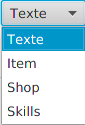
\includegraphics[width=1cm]{img/preludeListeDeroulante.png}
			\end{minipage}


			Cette onglet permet donc, par exemple, de décrire l'histoire du personnage ainsi que de choisir avec quel objets/compétences le joueur veut commencer. L'histoire peut alors changer en fonctions des objets/compétences que le joueur a en sa possession.
			Le bouton 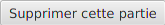
\includegraphics[height=10pt]{img/preludeSupprimerBouton.png} permet de supprimer le texte ainsi que sa particularité associé.

			\subsubsection{Particularité item et shop}\phantomsection \label{subsubsection:Item/Shop}
				Une liste déroulante s'affiche avec tout les items encore non sélectionné. Pour ajouter un item, il faut d'abord en sélectionner un, puis cliquer sur le bouton 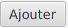
\includegraphics[height=10pt]{img/ajouterBouton.png}. Une fois l'item ajouter, il peut-être supprimé grâce à un clique droit sur l'item voulu.
				L'utilisateur peut aussi le sélectionner afin de renseigner des informations sur cette item:
				\begin{itemize}
					\item \textbf{Particularité Item} : le nombre d'item disponible peut être modifié grâce au champ disponible en bas.
					\item \textbf{Particularité Shop} : le nombre d'item disponible à la vente, ainsi que son prix d'achat et son prix de vente peuvent être modfié grâce aux champs en bas.
				\end{itemize}
				Si un champ est changé, l'utilisateur doit alors cliquer sur le bouton modifier pour valider le nombre.

			\subsubsection{Particularité compétence}\phantomsection \label{subsubsection:compétences}
				Le bouton 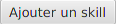
\includegraphics[height=10pt]{img/preludeAjouterSkillBouton.png} permet d'ajouter une liste déroulante. Chaque liste déroulante contient la liste des compétences disponible.

		\subsection{Personnage de base}
			Le personnage principal est créé ici. Son nom, ses points de vie, ses points de dégâts ainsi que la quantité d'items pouvant être porter et le nombre de monnaie possédé au départ peut alors être renseigné. Une coche est également présente afin de permettre à l'utilisateur de choisir si le personnage principal aura la possibilité de faire un double dégât ou non. La chance d'un double dommage est de 2/5.
			Si un champ contenant normalement un nombre est rempli par du texte, un message d'erreur aparait. Il en est de même si un champ n'est pas rempli.\\
		\newline
		Une fois l'onglet \textit{Personnage de base} rempli, l'utilisateur peut alors valider. Dans le cas contraire, un message d'erreur apparait. L'utilisateur peut aussi annuler. Aucune modification sera alors enregistré.

	\section{Les noeuds}
		La création d'un noeud se fait à partir du mode 
\includegraphics[height=10pt]{img/modeEdition.png}. Ce mode permet de créer un paragraphe. Une fois le mode sélectionné, il faut alors cliquer n'importe où dans la zone d'édition. Une fenêtre va alors apparaître.

		\subsection{Noeuds à choix}
			Ces noeuds contiennent trois onglets: édition du noeud (\textit{Noeud}), ajout des items à prendre (\textit{Item}), ajout des items à acheter (\textit{Shop}).

			\begin{itemize}
				\item \textbf{Noeud} : contient un paragraphe, un champ de texte de gain/perte de vie, un champ de texte permettant à l'utilisateur de définir un nombre maximum d'item à prendre/acheter sur ce noeud.
				\begin{center}
					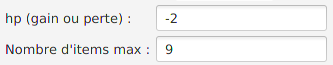
\includegraphics[height=1cm]{img/noeudBasic.png}
				\end{center}

				\item \textbf{Item} et \textbf{Shop} : voir la subsection \textbf{Particularité item et shop} \ref{subsubsection:Item/Shop} à la page \pageref{subsubsection:Item/Shop}. Des items doivent être créé pour être sélectionné (Voir le chapitre \ref{chapter:inclus} à la page \pageref{chapter:inclus}).
			\end{itemize}

			Tout les champs des noeuds, sauf le champ contenant le paragraphe (\textit{Texte}), ne peut contenir des lettres.

			\subsubsection{Noeud basic}
				Ce noeud permet d'avoir un simple paragraphe à choix.

			\subsubsection{Noeud aléatoire}
				Ce noeud ne diffère pas du noeud basique sur sa présentation, mais à la création de son/ses lien(s) (voir la section \ref{subsection:lienAléatoire} à la page \pageref{subsection:lienAléatoire}).

			\subsubsection{Noeud combat}\phantomsection\label{subsubsection:combat}
				Ce noeud contient deux nouvelle données à remplir. Tout d'abord, l'utilisateu peut définir le nombre de tours avant évasion. Puis il y a un bouton 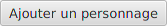
\includegraphics[height=10pt]{img/noeudAddPersonnage} permettant d'ajouter des ennemis grâce à une liste déroulante qui apparait. Chaque ennemis peut être ajouter plusieurs fois permettant ainsi de laisser la liberté à l'utilisateur d'avoir plusieurs même ennemis. Pour choisir un ennemis, il doit d'abord être créé (Voir le chapitre \ref{chapter:inclus} à la page \pageref{chapter:inclus})
				Ce noeud diffère également lors de la création de son/ses lien(s) (voir la section \ref{subsection:lienCombat} à la page \pageref{subsection:lienCombat}).

		\subsection{Noeud terminaux}
			Ces noeuds permettent de définir si le joueur a gagné ou perdu. Le livre est donc fini à cette endroit. Le livre ne peut pas être lancé tant que tout les noeuds ne finissent pas sur un noeud terminal. En effet, il est impossible au joueur de terminer sur un autre noeud qu'un noeud terminal.

	\section{Modification des noeuds}
		Ces différents noeuds présentés sont modifiables à l'aide du mode 
\includegraphics[height=0.4cm]{img/modeSelected.png}. Un double clique est nécessaire afin de pouvoir éditer le noeud voulu.

	\section{Positionnement des noeuds}
		Les noeuds peuvent être déplacés grâce au mode 
\includegraphics[height=10pt]{img/modeSelected.png}. Un simple clique/glisse suffit pour déplacer n'importe quel noeud.

	\section{Supression des noeuds}
		Ces noeuds, sauf le prélude, peuveut être supprimés à l'aide du mode 
\includegraphics[height=0.4cm]{img/modeSupression.png}. Un simple clique sur le noeud est alors necessaire. Une boite de dialog va alors s'ouvrir permettant de vérifier si l'utilisateur est bien sûr de son action. Attention, si des liens étaient présent sur ce noeud, ils sont tout simplement supprimés.
